\begin{savequote}[75mm]
This is some random quote to start off the chapter.
\qauthor{Firstname lastname}
\end{savequote}

\chapter{The ATLAS detector and the Large Hadron Collider}

This chapter presents an overview of the experimental systems used to conduct the measurements presented in this thesis. First, a brief overview of the accelerator, the Large Hadron Collider, will be given. In this section, the accelerator conditions relevant to data-taking are presented as well. Next, an overview of the ATLAS experiment is given. The basics of each sub-detector's role are summarized, as well as the details of the datasets accumulated. Then, a brief interlude on the ATLAS Muon New Small Wheel upgrade is presented. While this new detector does not have a direct impact on any of the datasets taken so far, it will have an impact on future analyses and the work done on it is briefly summarized here. Finally, an overview of object reconstruction in ATLAS is given. While the details of all of the algorithms will not be presented in detail, aspects of the reconstruction performance such as object resolutions are shown as these are relevant to the two studies presented later in this thesis. 

\section{The Large Hadron Collider}

The Large Hadron Collider (LHC) is a proton-proton collider at the CERN laboratory in Geneva, Switzerland\cite{LHCPaper}. It is designed for a maximum collision center of mass energy of $\sqrt{s} = 14 \TeV$ and has a circumference of $26.7$ kilometers. Four main experiments are located at the interaction points (IP) of the accelerator: ATLAS (A Toroidal LHC ApparatuS), CMS (the Compact Muon Solenoid), ALICE (A Large Ion Collider Experiment), and LHC$b$~\cite{ATLASPaper, CMSPaper, LHCbPaper, ALICEPaper}. The studies performed in this thesis were all completed with the ATLAS detector.

Figure~\ref{fig:LHC} shows a schematic of the LHC ring and the various experiments.  

\begin{figure}[h!]
  %\vspace{20pt}
  \centering
  \captionsetup{justification=centering}

  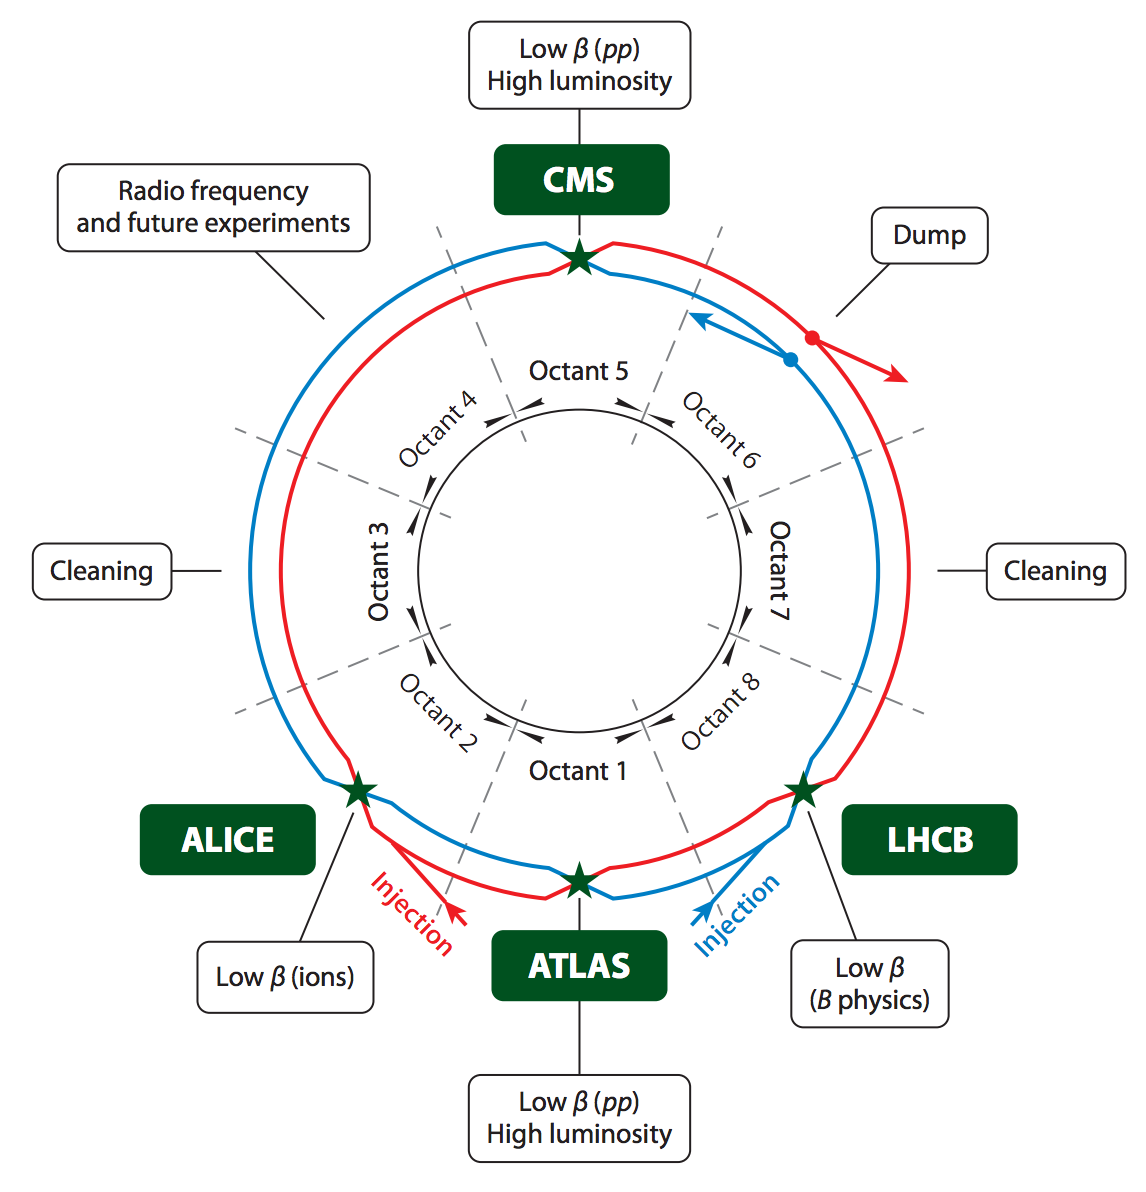
\includegraphics[width=0.7\textwidth]{figures/LHC}
   \caption{A schematic view of the LHC ring ~\cite{LHCReview}}
  \label{fig:LHC}
\end{figure}

\subsection{Instantaneous luminosity}

The rate of physics events expected from the accelerator is dependent on the instantaneous luminosity of the machine and the cross section of the physics process, $R_{\rm events} = L\sigma$. Here, $R_{\rm events}$ is the number of events per second, $L$ is the instantaneous luminosity of the machine, and $\sigma$ is the cross section for the physics process being measured. The instantaneous luminosity of the LHC is determined by numerous factors related to machine conditions. Equation~\ref{eqn:lumi} gives the equation for instantaneous luminosity of Gaussian beam profile~\cite{LHCReview}.

\begin{equation}
\label{eqn:lumi}
L = \frac{N_b^2 n_b f_{\rm rev} \gamma_r}{4\pi \epsilon_n \beta^*} F
\end{equation}

The LHC collides protons in bunches, and in the above equation $N_b$ is the number of protons per bunch while $n_b$ is the number of bunches per beam. Nominally, the LHC can hold up to $2808$ proton bunches. $f_{\rm rev}$ is the revolution frequency. $\epsilon_n$ is the normalized transverse beam emittance, a measurement of the average spread of the particles position-momentum space which has the dimension of length. $\beta^*$ is the value of the $beta$ function for the beam at the interaction point. It relates the emmitance to the Gaussian width of the beam with $\sigma_{\rm beam} = \sqrt{\epsilon \cdot \beta}$. $F$ is a reduction factor that corrects for the fact that the beams are colliding at an angle at the IP. 




\section{The ATLAS Detector}

\section{The ATLAS New Small Wheel Muon Upgrade}

\section{Object Reconstruction in ATLAS}
